\chapter{为什么需要量子天文学}
\label{chap:02}

\begin{chapteropening}
普通天文学已经能给出图像、光谱、光变曲线和偏振。那为什么还需要“量子天文学”？本章要回答的核心问题是：当我们把光子事件压缩成平均强度以后，是否还有物理信息被丢掉了？

答案是有。平均强度告诉我们“有多少光”，但不一定告诉我们“这些光子怎样一起到达”。量子天文学不否定传统数据产品，而是回到更底层的光子事件表，保留到达时间、望远镜位置、频率、偏振和事件之间的联合概率。HBT、Narrabri、恒星 photon bunching、VERITAS 和 MAGIC 强度干涉已经说明，这类信息可以真实测量；它既不等同于量子引力，也不只是把光子一个个数出来 \citep{1956Natur.178.1046H,1974iiia.book.....H,2017MNRAS.472.4126G,2020NatAs...4.1164A,2024MNRAS.529.4387A}。
\end{chapteropening}

\section{普通天文学为什么会丢掉一部分信息}
\label{sec:2-classical-products}
\label{sec:2-lost-correlations}

第 \ref{chap:01} 章把一次光子探测写成事件行 \(e_j=(t_j,\bm r_j,\nu_j,p_j,w_j)\)。这里 \(t_j\) 是到达时间，\(\bm r_j\) 是接收位置或望远镜编号，\(\nu_j\) 是频率通道，\(p_j\) 是偏振标签，\(w_j\) 是权重。现在的问题是：当我们把这张表变成一幅图像、一条光谱或一条光变曲线时，哪些列被保留，哪些关系被平均掉？

先看最熟悉的图像。若把事件按角坐标 \((x,y)\) 分箱，像素面积为 \(\Delta\Omega\)，曝光时间为 \(\Delta t\)，频率带宽为 \(\Delta\nu\)，则该像素的平均亮度可估计为
\begin{equation}
  \hat I(x,y)\simeq
  \frac{N(x,y)}
       {A_{\rm eff}\,\eta\,\Delta t\,\Delta\nu\,\Delta\Omega}.
  \label{eq:ch02-image-intensity}
\end{equation}
\begin{formulaexplain}
\(\hat I(x,y)\) 是像素亮度估计；\(N(x,y)\) 是该像素光子数；\(A_{\rm eff}\)、\(\eta\)、\(\Delta t\)、\(\Delta\nu\)、\(\Delta\Omega\) 分别给出收集面积、效率、曝光时间、带宽和立体角。它说明普通图像把事件表压缩成一阶平均量。
\end{formulaexplain}
这里 \(N(x,y)\) 是该像素内的加权光子数；\(A_{\rm eff}\) 是有效收集面积，单位 \(\mathrm{cm^2}\)；\(\eta\) 是系统总效率；\(\Delta\Omega\) 的单位是 sr。这个公式做了一件很自然的事：把一个像素里的事件全部加起来，再除以收集面积、效率、时间、带宽和立体角。光谱是按 \(\nu\) 分箱，光变曲线是按 \(t\) 分箱，普通偏振是把不同偏振通道的平均强度组合成 Stokes 参数。它们都主要是一阶统计量。

一阶统计量回答的是“单个事件落在哪里”或“某个 bin 里总共有多少事件”。它不回答“两个事件是否倾向于一起出现”。例如，把 \(10^8\) 个事件压缩成一条光变曲线以后，我们仍然知道每个时间 bin 的总数，却不知道同一 bin 里的事件是否成对聚集、是否来自同一对望远镜、是否落在同一频率和偏振模式中。对许多天体物理问题，这种压缩完全足够；但对强度干涉、光子聚束、跨谱线相关、偏振相关和最优参数估计，它会把目标信号本身压掉。

\begin{figure}[tbp]
\centering
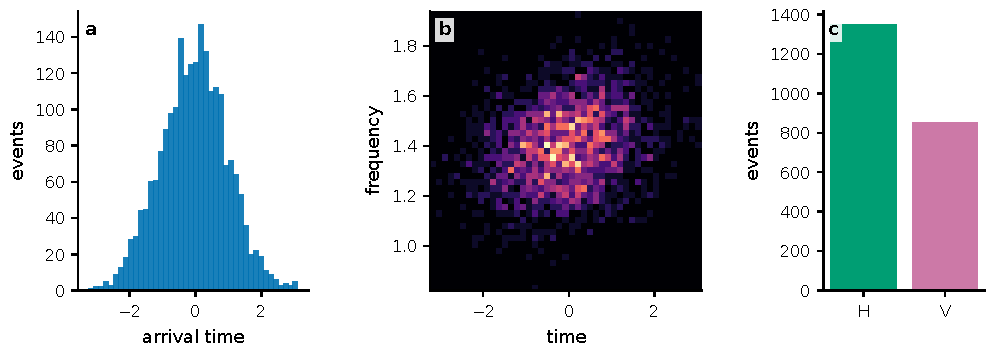
\includegraphics[width=0.92\linewidth]{figures/generated/chapter_02/ch02_event_table_information.pdf}
\caption{光子事件表把时间、望远镜位置、频率通道和偏振标签放在同一个数据结构中。按单一坐标边缘化得到光变曲线、谱线或偏振强度；保留两两事件关系则得到延迟直方图、强度相关函数和跨通道协方差。}
\label{fig:chapter-02-event-table}
\end{figure}

图 \ref{fig:chapter-02-event-table} 给出了这件事的数据图像。只保留单事件分布时，我们得到传统数据产品；保留事件对时，才开始看到延迟直方图、强度相关函数和跨通道协方差。量子天文学的第一个动机正是在这里：它不是先假设光有多“神秘”，而是先问事件表里是否有传统平均量没有使用的信息。

一个简单例子能说明这个差别。两束光可以有相同的平均强度和相同的光变曲线，但短时间延迟上的事件对数量不同。Poisson 光的到达近似彼此独立；热光在相干时间内有过量共同到达概率。这两者的平均亮度可以一样，但二阶统计不同。因此下一步要理解的不是“更多光子数”，而是“事件之间的联合概率”。

\section{怎样把“光子一起到达”写成可测量的量}
\label{sec:2-thermal-coherent}

物理上，相关就是“一个事件发生后，另一个事件发生的概率是否改变”。用 \(a\) 表示一个事件标签，它可以是时间 bin、望远镜编号、频率通道或偏振通道。一阶概率 \(P_1(a)\) 描述单个事件落入 \(a\) 的概率；二阶概率 \(P_2(a,b)\) 描述两个事件分别落入 \(a\) 和 \(b\) 的联合概率。若事件完全独立，就有
\begin{equation}
  P_2(a,b)=P_1(a)P_1(b).
  \label{eq:ch02-independent}
\end{equation}
\begin{formulaexplain}
\(P_1(a)\) 和 \(P_1(b)\) 是单事件概率；\(P_2(a,b)\) 是两个事件的联合概率。乘积形式表示完全独立到达；任何偏离它的部分才是相关信号。
\end{formulaexplain}
这条公式是“没有相关”的基线。任何偏离这个乘积的部分，都说明事件之间存在额外关系。

在实际数据里，我们通常数某个时间窗或某个延迟下的事件数。令 \(N_a\) 和 \(N_b\) 是两个通道中的计数，最直接的共同涨落量是协方差
\begin{equation}
  C_{ab}=\langle N_aN_b\rangle-\langle N_a\rangle\langle N_b\rangle.
  \label{eq:ch02-cov}
\end{equation}
\begin{formulaexplain}
\(C_{ab}\) 是通道 \(a,b\) 的协方差；\(N_a,N_b\) 是计数；第一项是真实共同涨落，第二项是独立到达时的平均乘积。它把“是否一起变亮或变暗”写成可测量的差值。
\end{formulaexplain}
尖括号表示对许多时间窗、许多实验重复或许多统计等价样本求平均。第一项 \(\langle N_aN_b\rangle\) 是实际共同出现的平均乘积；第二项是如果两个通道只按各自平均率独立到达时的期望。若 \(C_{ab}=0\)，通道间没有可测共同涨落；若 \(C_{ab}>0\)，有过量共同到达；若 \(C_{ab}<0\)，可能是死时间、pile-up、选择效应，也可能是更特殊的反聚束。

为了把不同亮度的源放在同一尺度上，常用归一化二阶相关函数
\begin{equation}
  g^{(2)}_{ab}(\tau)=
  \frac{\langle N_a(t)N_b(t+\tau)\rangle}
       {\langle N_a(t)\rangle\langle N_b(t+\tau)\rangle}.
  \label{eq:ch02-g2-count}
\end{equation}
\begin{formulaexplain}
\(g^{(2)}_{ab}(\tau)\) 是延迟 \(\tau\) 下的归一化二阶相关；分子数跨通道事件对，分母给出随机符合基线。它把不同亮度、不同计数率的数据放到同一相关尺度上。
\end{formulaexplain}
\(\tau\) 是两个通道之间的延迟，单位秒。这个量可以从事件表直接估计：构造 \(a\) 通道和 \(b\) 通道的事件对延迟直方图，再除以由两个单通道平均计数率给出的随机符合。\(g^{(2)}=1\) 是独立到达；\(g^{(2)}>1\) 表示聚束或共同涨落；\(g^{(2)}<1\) 则必须同时考虑非经典反聚束和仪器效应。

有了这个归一化尺度，前面那个“平均亮度相同、事件关系不同”的例子就可以画出来。两束光在一阶统计上可以完全一样：同样的平均强度，同样的慢变光变曲线，同样的总光子数。但如果一束光的事件近似独立到达，另一束光在相干时间内更容易成对到达，它们的 \(g^{(2)}\) 曲线就不同。

\begin{figure}[tbp]
\centering
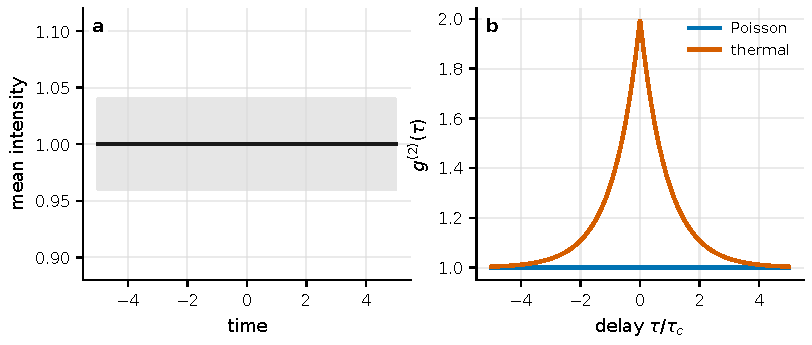
\includegraphics[width=0.92\linewidth]{figures/generated/chapter_02/ch02_mean_intensity_vs_correlation.pdf}
\caption{两束光可以有相同平均强度，却有不同的二阶相关函数。Poisson 光的 \(g^{(2)}\) 近似为 1；热光在相干时间内有过量共同到达概率，表现为 \(g^{(2)}(0)>1\)。}
\label{fig:chapter-02-mean-vs-correlation}
\end{figure}

这种差别来自光场状态本身。理想相干光的到达近似 Poisson 过程，知道平均率以后，一个光子的到来不改变同一模式中下一个光子的即时到达概率，因此零延迟相关为 1。单模热光有额外强度涨落：场强偏高的一小段时间里，多个光子都会更容易到达，于是零延迟附近的事件对多于随机基线，理想极限为 2。单模成对因子 \(b_2\) 给出这两个基准值，见式 \eqref{eq:ch03-coherent} 和式 \eqref{eq:ch03-thermal-density}；事件表中的归一化二阶相关把同一物理写成 \(g^{(2)}\)。

真实天体观测很少只收集一个模式。频率带宽、时间门宽、空间模式、偏振和背景都会把许多独立涨落平均到一起，使 \(g^{(2)}-1\) 变小。最重要的直觉是：随机符合基线随总光子数快速增长，真正携带聚束信息的同模涨落只占其中很小一部分。相干时间大约由光学带宽决定，带宽越宽，相干时间越短；若探测器或分析 bin 远慢于相干时间，聚束峰会被平均到 \(10^{-3}\)、\(10^{-6}\) 甚至更低。多模和时间响应的定量写法放在第 \ref{chap:04} 章式 \eqref{eq:ch04-multimode} 和式 \eqref{eq:ch04-contrast-dilution}。

\begin{figure}[tbp]
\centering
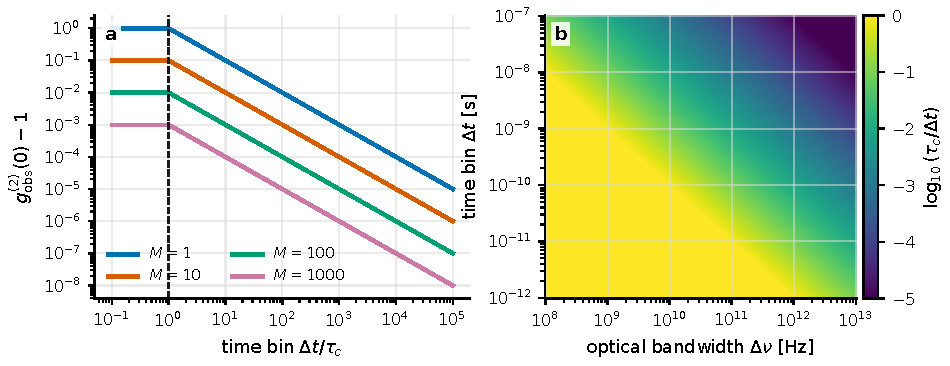
\includegraphics[width=0.92\linewidth]{figures/generated/chapter_02/ch02_contrast_dilution.pdf}
\caption{二阶相关对比度会被有效模式数和时间分辨率同时压低。左图显示模式数 \(M\) 增大或时间 bin \(\Delta t\) 大于相干时间 \(\tau_c\) 后，\(g^{(2)}_{\rm obs}(0)-1\) 快速下降。右图把 \(\tau_c\simeq1/\Delta\nu\) 代入，显示宽光学带宽和慢电子响应会把聚束峰压到很小。}
\label{fig:chapter-02-dilution}
\end{figure}

图 \ref{fig:chapter-02-dilution} 给出望远镜里的数量级。若 \(\Delta\nu=10^{12}\,\mathrm{Hz}\)，则 \(\tau_c\sim1\,\mathrm{ps}\)；若电子响应是 \(1\,\mathrm{ns}\)，即使是单模、单偏振热光，相关峰也只剩约 \(10^{-3}\)。再乘上多模、背景和偏振稀释，天文数据中的目标信号常常低到 \(10^{-6}\) 到 \(10^{-3}\)。这解释了为什么强度相关不是“看起来相关就行”，而是一项严肃的误差预算问题。

\section{HBT 为什么能测天体大小，又为什么长期困难}
\label{sec:2-hbt-history}
\label{sec:2-revival}

到这里我们知道了二阶相关能测“共同涨落”。HBT 是 Hanbury Brown--Twiss 的缩写，来自 R. Hanbury Brown 和 R. Q. Twiss 在 1950 年代提出并验证的强度干涉思想。这个想法先在实验室 photon correlation 中引起争论和确认，随后被用于 Sirius 的恒星测试，最后发展成 Narrabri Stellar Intensity Interferometer，并给出一批明亮恒星的角直径 \citep{1956Natur.177...27B,1957RSPSA.242..300B,1956Natur.178.1046H,1958RSPSA.248..222B,1974iiia.book.....H}。

把两台望远镜想成两个相距很远的光子计数器，它们都指向同一颗恒星。恒星表面的每一个小面元都像一个很小的热光源，发出的电场相位快速而随机地抖动。来自同一个小面元的光会同时到达两台望远镜，只是到达第二台时多走了一点路，因此多带一个几何相位。来自另一个小面元的光也会同时到达两台望远镜，但它的几何相位又不同。

如果恒星在这条基线上看起来很小，所有小面元给出的几何相位差几乎一样，两台望远镜收到的电场仍然很相似。如果恒星已经被分辨，不同小面元给出的相位差分散开，平均时互相抵消，两台望远镜收到的电场相似度就下降。角直径的信息就藏在这个下降速度里：基线越长，越容易看出恒星不是一个点。

普通振幅干涉把两路光在光学上合并，让电场相加，再从条纹对比度读出这种相似度。HBT 保留两路光各自的探测记录，然后比较两路光强涨落是不是同步。同步得强，说明两台望远镜接收到的热光模式仍然相似；同步得弱，说明这条基线已经分辨了源的角结构。

现在把“电场相似度”写成一个量。若第 \(i,j\) 个接收位置的窄带复电场分别为 \(E_i(t)\) 和 \(E_j(t)\)，一阶互相干函数和归一化一阶相干度定义为
\begin{equation}
  \begin{aligned}
    \Gamma^{(1)}_{ij}(\tau)
    &=
    \langle E_i^*(t)E_j(t+\tau)\rangle,\\
    \gamma^{(1)}_{ij}(\tau)
    &=
    \frac{\Gamma^{(1)}_{ij}(\tau)}
         {\sqrt{\Gamma^{(1)}_{ii}(0)\Gamma^{(1)}_{jj}(0)}},\\
    \langle I_i\rangle
    &=
    \kappa_i\,\Gamma^{(1)}_{ii}(0).
  \end{aligned}
  \label{eq:ch02-first-order-coherence}
\end{equation}
\begin{formulaexplain}
\(\Gamma^{(1)}_{ij}\) 是两处电场的互相关；\(\gamma^{(1)}_{ij}\) 是归一化的一阶相干度；\(\langle I_i\rangle\) 是第 \(i\) 路观测到的平均光强；\(\kappa_i\) 把场强平方换成探测器记录的光强或计数率。
\end{formulaexplain}
式 \eqref{eq:ch02-first-order-coherence} 的读法很直接。\(\Gamma^{(1)}_{ij}\) 把两处电场相乘再平均；两处电场的相位关系越稳定，平均后留下的量越大。对角项 \(\Gamma^{(1)}_{ii}(0)=\langle E_i^*(t)E_i(t)\rangle\) 是第 \(i\) 路平均光强对应的场强平方平均；探测器真正记录的是 \(\langle I_i\rangle\)，两者只差效率、带宽、增益和单位选择等比例因子。分母用两个对角项归一化，\(\gamma^{(1)}_{ij}\) 便只保留相干性的大小和相位。对两台望远镜取 \(i=1,j=2\)，\(|\gamma^{(1)}_{12}|=1\) 表示两处电场完全相干，\(|\gamma^{(1)}_{12}|=0\) 表示平均后没有共同相位关系留下。

\(\gamma^{(1)}_{12}\) 可以由振幅干涉测到，条件是仪器保存两路电场并把它们合并。单路探测器只给出 \(\Gamma^{(1)}_{11}(0)\) 或 \(\Gamma^{(1)}_{22}(0)\) 这样的平均强度项；两束光相加后，输出光强里会出现交叉项。若在其中一路加入可控相位 \(\varphi\)，合并后的平均光强可写成
\[
  I_{\rm comb}(\varphi)
  \propto
  \Gamma^{(1)}_{11}(0)+\Gamma^{(1)}_{22}(0)
  +2\,{\rm Re}\!\left[e^{i\varphi}\Gamma^{(1)}_{12}(0)\right].
\]
改变 \(\varphi\) 时，条纹对比度给出 \(|\gamma^{(1)}_{12}|\)，条纹位置给出 \(\arg\gamma^{(1)}_{12}\)。所以普通光学或射电振幅干涉测到的复可见度，本质上就是 \(\gamma^{(1)}_{12}\)。

HBT 的数据流不同。每台望远镜先把光变成光电流或光子事件表；随后把几何延迟校正掉，再问一个非常具体的问题：第一路在某个时刻偏亮时，第二路在相同延迟处是否也偏亮？连续光电流可以相乘平均；光子事件表则构造两路事件对的延迟直方图，再除以同样计数率和同样 live time 下的随机符合数。这个估计量的完整写法放在第 \ref{chap:04} 章式 \eqref{eq:ch04-g2-estimator}。

热光有一个关键性质：同一个模式会一阵亮、一阵暗。两台望远镜若接收到相干的同一批模式，就会一起看到这些亮暗起伏；两处电场越相似，强度涨落越同步。对高斯混沌热光，这句话由 Siegert 关系定量表达：强度相关的 excess 正比于一阶相干度的模平方。它的四阶矩推导见第 \ref{chap:04} 章式 \eqref{eq:ch04-siegert}；在空间 HBT 中，对应关系见第 \ref{chap:05} 章式 \eqref{eq:ch05-hbt-spatial}。物理读法是：HBT 从光强涨落读出的量，正是普通振幅干涉会称为“可见度”的模平方，真实观测还要乘上时间响应、模式、偏振和背景稀释因子。

还差最后一步：\(\gamma^{(1)}_{12}\) 为什么包含恒星大小？把恒星表面分成许多小面元。每个面元都像一个很小的点源，来自不同面元的热光彼此独立；因此求平均时，只有“同一个面元到达两台望远镜”的相关项留下来。一个面元越亮，它留下的相关项权重越大；一个面元方向越偏，它的几何相位转得越快。把所有面元按亮度加权相加，就得到 van Cittert--Zernike 定理：空间相干度是天空亮度的归一化 Fourier 分量。第 \ref{chap:05} 章式 \eqref{eq:ch05-vcz} 会给出完整公式和适用边界。

这条关系让强度干涉能测角大小。若源很小，各面元的相位几乎排在一起，\(|\gamma^{(1)}_{12}|^2\) 接近 1；若源被基线分辨，不同方向的相位互相抵消，\(|\gamma^{(1)}_{12}|^2\) 随基线下降。均匀圆盘会给出熟悉的 Bessel 型可见度曲线，第一零点和下降速度直接编码角直径；具体公式、第一零点和非均匀模型放在第 \ref{chap:05} 章式 \eqref{eq:ch05-uniform-disk} 之后讨论。

Sirius 测试和 Narrabri 强度干涉仪把这个方法带入天文学。Narrabri 使用两台 6.5 m 光收集器，测量热星角直径，并最终给出 32 颗恒星的角直径目录；后续工作还讨论了边缘昏暗如何影响从均匀圆盘直径到真实恒星直径的修正 \citep{1956Natur.178.1046H,1967MNRAS.137..375H,1967MNRAS.137..393H,1974MNRAS.167..121H,1974MNRAS.167..475H,1974iiia.book.....H}。HBT 的影响也超出天文学。Baym 的综述从恒星讲到核碰撞，说明同样的二粒子相关思想可以把“源的空间尺度”映射到“相关函数的宽度” \citep{1998AcPPB..29.1839B,1990RvMP...62..553B}。

那为什么这种方法后来沉寂了很久？主要原因是信号太小。强度干涉的相关峰要从巨大的随机符合背景中捞出来；提高信噪比最直接的资源是更大的收集面积、更高的量子效率、更宽的电子带宽和更长的积分时间，而这些资源只会以不同速度改善误差。经典 SNR 标度式和观测设计用法放在第 \ref{chap:05} 章式 \eqref{eq:ch05-snr} 和第 \ref{chap:18} 章。它的物理含义是：HBT 放宽了光学相位稳定要求，却把压力转移到光子数、时间响应、背景和系统误差预算上。

现代复兴主要靠工程条件变化。大口径 Cherenkov 望远镜阵列提供了现成的大收集面积；PMT、APD、SPAD 和高速电子学可以在 ns 到 ps 尺度记录涨落；FPGA/GPU 和离线相关允许把多台望远镜的数据流复制到许多基线组合中；精密时间同步和数字延迟校正可以跟踪几何光程差，而不必把光学相位稳定到纳米尺度。Le Bohec--Holder、Dravins--CTA 和后来的 CTA 布局模拟给出的工程路线很一致：信号弱，但电子相关器可以复制，粗糙光学也能工作，多台望远镜会把 \(u,v\) 覆盖变成主要资产 \citep{2006ApJ...649..399L,2008AIPC..984..205L,2012NewAR..56..143D,2013APh....43..331D,2010SPIE.7734E..1CN,2010SPIE.7734E..1TJ}。

现代实测已经越过“概念可行”阶段。Guerin 等人用 1 m 望远镜在 photon-counting 模式下测到 Arcturus、Procyon 和 Pollux 的时间 photon bunching，相关峰对比度约 \(2\times10^{-3}\)，噪声接近 shot-noise 标度 \citep{2017MNRAS.472.4126G}。VERITAS 四台 12 m Cherenkov 望远镜的强度干涉系统测量了 \(\beta\) CMa 和 \(\epsilon\) Ori 的亚毫角秒角直径，精度优于 5\%，并展示了多基线离线相关的可扩展性 \citep{2020NatAs...4.1164A}。MAGIC 两台 17 m Cherenkov 望远镜也完成了光学强度干涉观测，后续系统论文给出了性能和第一批测量结果 \citep{2020MNRAS.491.1540A,2024MNRAS.529.4387A}。Aqueye/Iqueye 的 Vega photon-counting 实验则展示了高时间分辨事件表、零基线相关和公里级基线校准中的系统误差问题 \citep{2021MNRAS.506.1585Z}。

\begin{figure}[tbp]
\centering
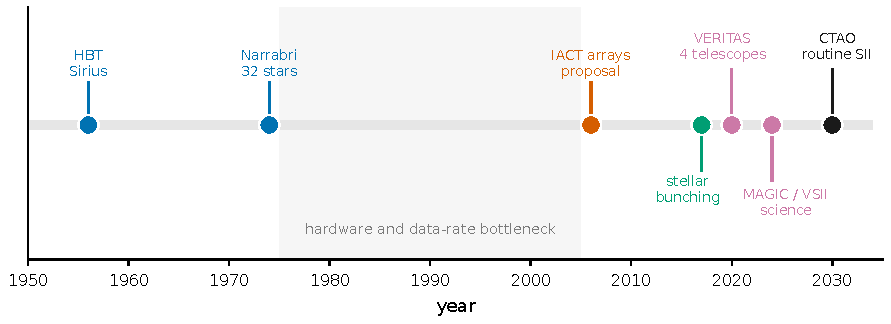
\includegraphics[width=0.92\linewidth]{figures/generated/chapter_02/ch02_revival_timeline.pdf}
\caption{光学强度干涉从 HBT 和 Narrabri 到 Cherenkov 阵列复兴的时间线。1970 年代之后的沉寂主要来自大面积光收集器、高速探测和多基线相关器的工程瓶颈；IACT 阵列、数字相关和 photon-counting 事件表把这些瓶颈逐步移开。}
\label{fig:ch02-revival-timeline}
\end{figure}

这条历史给本书一个很实际的判断：强度相关不是概念上不可行，而是需要足够光子数、足够稳定的时间系统、足够强的 null test 和足够诚实的误差预算。

\section{什么算量子天文学，第一代问题在哪里}
\label{sec:2-definition}
\label{sec:2-first-cases}

有了上面的例子，就可以给出本书的工作定义。量子天文学是一类事件层面的观测问题：研究天体光场的联合概率、相干函数和模式信息，并用这些量处理天体物理、传播效应、基础物理或观测设计。它的基本数据是带标签的光子事件表，而不只是平均强度数据产品。高速光子计时仪器如 Iqueye/Aqueye 的设计初衷，就是把天文光子作为带纳秒或更高时间精度的事件来处理 \citep{2010SPIE.7702E..0MC}。

更一般地，光电探测可以按一重、二重、三重乃至更高阶符合来组织。\(n=1\) 给出普通平均强度，\(n=2\) 给出 HBT 和 photon bunching，\(n=3\) 可在多望远镜强度干涉中帮助恢复部分相位信息。场算符和光态给出这些符合统计的量子来源；事件表和相关估计量给出它们的观测实现。它们都对应可估计的符合统计。

这个边界很实用。量子天文学不等于量子引力，也不等于任何使用“量子”二字的宇宙学讨论。一个问题若不能写成事件表中的可估计量、误差模型和 null test，就还不是可执行的观测项目。反过来，普通 photon counting 也不自动属于量子天文学；只有当单光子事件的联合统计、模式结构或最优测量比平均强度提供额外信息时，它才进入这个范围。

第一代最稳妥的科学目标是明亮恒星。强度干涉可以测角直径、边缘昏暗、快速自转引起的扁率、双星分离和热星风结构。恒星足够亮，近似热光，角尺度在 \(0.05\) 到数 mas，正好落在百米到公里级可见光基线的敏感范围。Narrabri 的历史结果、VERITAS/MAGIC 的现代直径测量、\(\beta\) UMa 角直径和 \(\gamma\) Cas 扁率结果，都把这类目标推到第一代观测的最前面 \citep{1974MNRAS.167..121H,2020NatAs...4.1164A,2024MNRAS.529.4387A,2024ApJ...966...28A,2025ApJ...995..191A}。

时间结构明显的源提供另一条路线。脉冲星、爆发源、nova、supernova 和微透镜事件把到达时间放到中心位置。若两个未分辨光路有微小时间延迟，photon bunching 的延迟结构可能携带额外信息。Saha 提出用 photon bunching 测微透镜质量，Lewis 和 Tuthill 随后讨论 decoherence 对这种设想的影响，说明这类想法需要同时处理相干时间、源尺寸和传播路径差 \citep{2019MNRAS.486.5400S,2020MNRAS.491.5789L}。

频率和偏振相关则把问题推向辐射机制。谱线内外的 \(g^{(2)}(\tau)\) 可以连接到相干时间和谱宽；偏振分辨相关可以测试辐射机制、磁场几何和传播效应。自然 laser 的 photon-correlation spectroscopy、黑体 photon bunching 和 X-ray driven photon bunching 都显示，HBT 思想不只属于恒星角直径，也可以成为谱线宽度、激发过程和高能闪烁的诊断工具 \citep{2005NewA...10..361J,2008AIPC..984..216D,2014ApJ...789L..10T,2024arXiv241216975K}。这些方向离常规巡天更远，但物理链条仍然从事件表开始，经过光子统计，再进入辐射机制、传播效应和基础物理。

\begin{figure}[tbp]
\centering
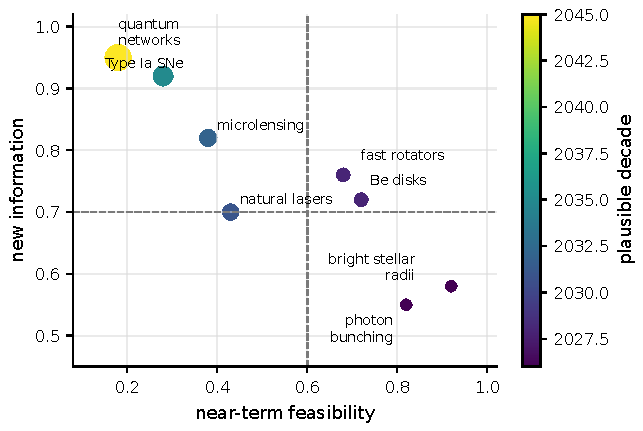
\includegraphics[width=0.76\linewidth]{figures/generated/chapter_02/ch02_science_case_map.pdf}
\caption{第一代量子天文学科学问题的可行性和新增信息量。亮星角直径和恒星 photon bunching 已经靠近常规观测；Be 星盘、快速自转星和自然 laser 属于近期扩展；Type Ia 超新星角距离和量子网络望远镜科学价值高，但需要更长基线、快速触发或量子链路工程。}
\label{fig:ch02-science-map}
\end{figure}

\begin{longtable}{p{0.22\linewidth}p{0.30\linewidth}p{0.36\linewidth}}
\toprule
观测量 & 典型范围 & 主要限制 \\
\midrule
\(R_\gamma\) & \(10^5\) 到 \(10^9\,\mathrm{s^{-1}}\) 对亮星单通道可达 & 探测器饱和、死时间、背景和数据率。 \\
\(\Delta t\) & \(10\,\mathrm{ps}\) 到 \(10\,\mathrm{ns}\) & 探测器抖动、电子带宽、镜面等时性和时钟同步。 \\
\(\Delta\nu\) & \(10^9\) 到 \(10^{13}\,\mathrm{Hz}\) & 窄带提高相干时间但降低光子率；宽带相反。 \\
\(g^{(2)}-1\) & \(10^{-6}\) 到 \(10^{-3}\) 常见于天文强度干涉 & 模式数、时间稀释、偏振稀释和背景稀释。 \\
\(B\) & \(10\,\mathrm{m}\) 到 \(10\,\mathrm{km}\) & 决定角尺度；长基线信号小，需要更多光子和更准模型。 \\
\(|\gamma^{(1)}|^2\) & 0 到 1 & 源被分辨后下降；只测模平方时相位恢复困难。 \\
\bottomrule
\end{longtable}
